% BÀI TOÁN HÌNH HỌC - BAI_HINH_14 (TRÍCH ĐỀ 14)
\begin{ex}
% Câu 13
	Cho đường tròn tâm $O$ đường kính $AB=2R$, trên đoạn $OA$ lấy điểm $I$ ($I \ne A; I \ne O$). Vẽ tia $Ix \perp AB$ cắt $(O)$ tại $C$. Lấy điểm $E$ trên cung nhỏ $BC$ ($E \ne B; E \ne C$), $AE$ cắt $CI$ tại $F$, gọi $D$ là giao điểm của $BC$ với tiếp tuyến tại $A$ của $(O;R)$.
	\begin{enumerate}
		\item[a)] Chứng minh rằng tứ giác $BEFI$ là tứ giác nội tiếp.
		\item[b)] Chứng minh rằng $AE \cdot AF = CB \cdot CD$. Biết rằng $AB=2AC$, tia $Iy$ là tia đối của tia $Ix$ cắt đường tròn $(O)$ tại điểm $M$. Tìm giá trị lớn nhất của biểu thức $S = 2025 \cdot EB \cdot EC$.
	\end{enumerate}
\loigiai{
{
		\begin{center}
		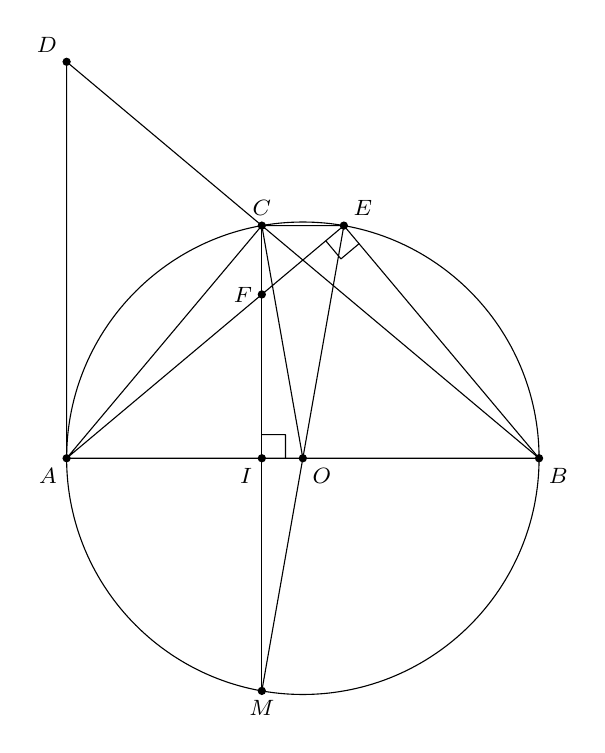
\begin{tikzpicture}[line join = round, line cap=round,>=stealth,font=\footnotesize,scale=1]
			\usetikzlibrary{calc,intersections,angles}
			
			% Khai báo hằng số
			\def\r{3} % r = 3cm
			\def\aConstant{4} % a = 4 (Lưu ý: hằng số a này không được sử dụng trong các định nghĩa điểm mới)
			\def\alphaAngle{100} % alpha = 100 độ
			
			% Định nghĩa tọa độ các điểm
			\coordinate (O) at (0,0);
			\coordinate (A) at (-\r,0);
			\coordinate (B) at (\r,0);
			% D(-r; 2r*tan(90-alpha/2))
			\pgfmathsetmacro{\yDVal}{2*\r*tan(90-\alphaAngle/2)}
			\coordinate (D) at (-\r,\yDVal);
			
			% Tọa độ cực C(alpha;r), E(80;r)
			\coordinate (C) at (\alphaAngle:\r);
			\coordinate (E) at (80:\r);
			
			% I là hình chiếu của C lên AB (trục Ox)
			% Cx = r*cos(alphaAngle), Cy = r*sin(alphaAngle)
			% Ix = Cx, Iy = 0
			\pgfmathsetmacro{\CxVal}{\r*cos(\alphaAngle)}
			\pgfmathsetmacro{\CyVal}{\r*sin(\alphaAngle)}
			\coordinate (I) at (\CxVal,0);
			
			% Lấy điểm M sao cho I là trung điểm của CM
			% Mx = 2*Ix - Cx = Ix
			% My = 2*Iy - Cy = -Cy
			\coordinate (M) at (\CxVal,-\CyVal);
			
			% AE cắt CM tại F
			\path[name path=lineAE_F] (A) -- (E);
			\path[name path=lineCM_F] (C) -- (M);
			\path[name intersections={of=lineAE_F and lineCM_F, by=F}];
			
			% Vẽ các đối tượng hình học
			\draw (O) circle (\r);          % Đường tròn (O;r)
			\draw (A) -- (D) -- (B) -- cycle; % Tam giác ADB (A-D-B-A)
			\draw (C) -- (M);               % Đoạn C-M
			\draw (O) -- (C);               % Đoạn O-C
			\draw (B)--(E)--(A) -- (C) -- (E) -- (M); % Đường A-C-E-M (Lưu ý: không đóng thành cycle)
			
			% Tô màu cho các điểm (theo cấu trúc đầu tiên)
			\fill (O) circle (1.5pt);
			\fill (A) circle (1.5pt);
			\fill (B) circle (1.5pt);
			\fill (D) circle (1.5pt);
			\fill (C) circle (1.5pt);
			\fill (E) circle (1.5pt);
			\fill (I) circle (1.5pt);
			\fill (M) circle (1.5pt);
			\fill (F) circle (1.5pt);
			
			% Đặt nhãn cho các điểm (theo cấu trúc đầu tiên)
			\node[below right] at (O) {$O$};
			\node[below left] at (A) {$A$};
			\node[below right] at (B) {$B$};
			\node[above left] at (D) {$D$};
			\node[above] at (C) {$C$}; % Vị trí tương đối
			\node[above right] at (E) {$E$}; % Vị trí tương đối
			\node[below left] at (I) {$I$};
			\node[below] at (M) {$M$}; % Vị trí tương đối
			\node[left] at (F) {$F$};   % Vị trí tương đối
			
			% Không có yêu cầu ký hiệu góc vuông trong lần này
			\pic[draw, angle radius=3mm]{right angle = F--I--B};
			\pic[draw, angle radius=3mm]{right angle = F--E--B};
		\end{tikzpicture}
		
		\end{center}
}
\end{ex}
